\chapter{Requisiti}
Al fine di applicare le tecnologie che tratteremo nel capitolo 4, mi è stato richiesto di sviluppare una web app.
La web app deve implementare i seguenti requisiti:
\begin{itemize} 
    \item Pagina di login: pagina in cui l'utente può autenticarsi utilizzando il proprio username e password. La password deve essere crittografata nel database utilizzando la funzione crittografica di hash Bcrypt. Inoltre ad ogni utente deve essere associato un ruolo, che viene usato per gestire i permessi di accesso alle pagine della web app. Se l'utente non ha i permessi per accedere a un determinato endpoint, quest'ultimo deve essere mandato alla pagina di accesso negato. Mentre se possiede il ruolo "EMPLOYEE" viene mandato alla home page (postit-home). (Figura \ref{fig:pagine})
    \item Homepage: pagina in cui è presente una navbar, nella quale viene mostrato il titolo della web app, l'username e il ruolo dell'utente autenticato. All'interno della navbar devono essere presenti due bottoni, uno per la creazione dei postit, l'altro per effettuare il logout.
    Inoltre sotto la navbar vengono visualizzate delle note, chiamate postit, le quali sono costituite da un titolo e descrizione. Ogni postit deve avere la possibilità di essere modificato ed eliminato.
\end{itemize}
\begin{figure}[h]
    \centering
    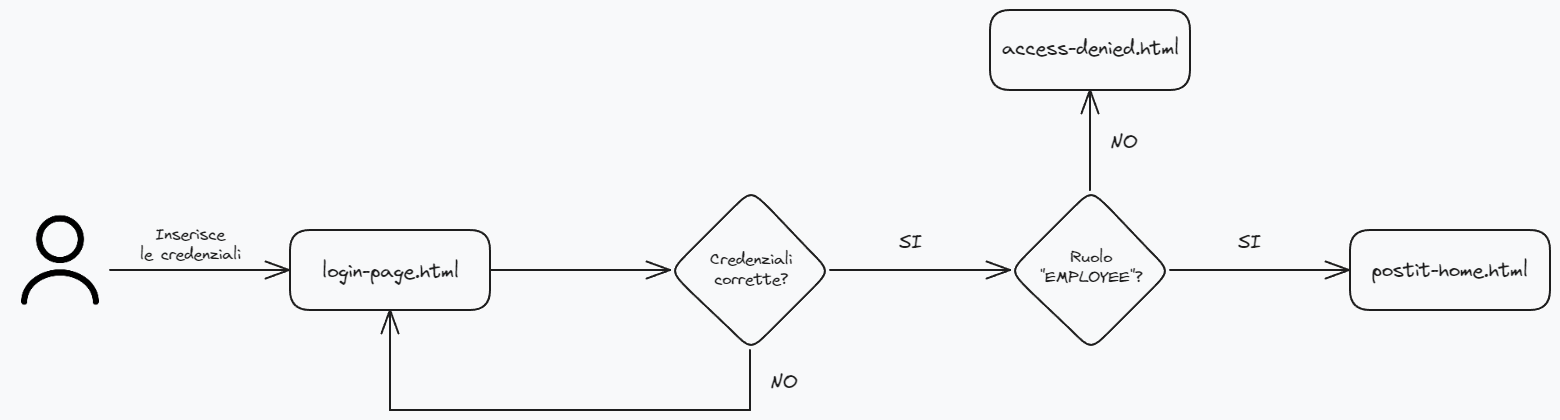
\includegraphics[width=1.0\textwidth]{images/funzionamento pagine.png}
    \caption{Pagine da implementare}
    \label{fig:pagine}
\end{figure}
\newpage
\subsubsection{Back-end}
Il back-end deve essere implementato basandosi sul pattern MVC, utilizzando il framework Spring Boot, andando a implementare:
\begin{itemize}
    \item Entità postit;
    \item Controller per login e home page;
    \item Configurazione per la gestione della sicurezza al fine di gestire l'autenticazione degli utenti e i permessi di accesso alle pagine di questi ultimi.
\end{itemize}
\subsubsection{Front-end}
Il front-end deve implementare le seguenti pagine:
\begin{itemize}
    \item login-page.html, la quale deve avere uno stile css;
    \item postit-home.html, la quale deve avere uno stile css usando il framework bootstrap;
    \item access-deniend.html
\end{itemize}
\subsubsection{Database}
I dati devono essere mantenuti all'interno di un database.
Il database, PostgreSQL, deve essere inserito in un container utilizzando l'applicativo Docker, e deve implementare le seguenti tabelle:
\begin{itemize}
    \item users
    \item ruoli
    \item postit
\end{itemize}
Al fine di recuperare i dati dal back-end e mostrarli nel front-end deve essere utilizzato il motore di template Thymeleaf.
